\documentclass[10pt,letterpaper]{article}
\usepackage[T1]{fontenc}
\usepackage[utf8]{inputenc}
\usepackage{lmodern}
\usepackage[margin=0.8in,top=0.7in,bottom=0.75in]{geometry}
\usepackage{microtype}
\usepackage{amsmath}
\usepackage{xcolor}
\usepackage{graphicx}
\usepackage{tikz}
\usetikzlibrary{arrows.meta,positioning,calc}
\usepackage{booktabs}
\usepackage{tabularx}
\usepackage{array}
\usepackage{float}
\usepackage{caption}
\usepackage{hyperref}

\definecolor{ours}{HTML}{1F5FA8}
\definecolor{oursfill}{HTML}{E3EDF8}
\definecolor{pre}{HTML}{6B6B6B}
\definecolor{prefill}{HTML}{EFEFEF}
\definecolor{ink}{HTML}{4A3F38}
\definecolor{bystander}{HTML}{8A7A6C}
\definecolor{matched}{HTML}{7C8794}
\definecolor{wall}{HTML}{F6F1E6}
\definecolor{floorc}{HTML}{D8CBB3}

\hypersetup{colorlinks=true,urlcolor=ours,linkcolor=black,citecolor=black}
\captionsetup{font=small,labelfont=bf,skip=4pt}
\setlength{\parindent}{0pt}
\setlength{\parskip}{4.2pt}
% Figures are placed by hand on the two figure pages, so keep their own margins small.
\setlength{\intextsep}{4pt}
\pagestyle{empty}
\frenchspacing
\graphicspath{{figures/}}

% ---------- a standing figure for Figure 5 ----------
% #1 centre x, #2 height of the soles, #3 scale, #4 colour, #5 right arm: down or raised
\newcommand{\person}[5]{%
  \begin{scope}[shift={(#1,#2)},scale=#3]
    \draw[#4,line width=#3*2.7pt] (-3.1,20.8) -- (-3.8,0) (3.2,20.8) -- (3.9,0);
    \draw[#4,line width=#3*2.38pt] (-6.1,36.1) -- (-11.7,21.7);
    \ifx#5r
      \draw[#4,line width=#3*2.7pt] (6.1,36.1) -- (14.0,42.6) -- (22.2,55.1);
    \else
      \draw[#4,line width=#3*2.38pt] (6.1,36.1) -- (11.8,21.7);
    \fi
    \fill[#4,rounded corners=#3*1.3pt] (-5.5,38.4) -- (5.5,38.4) -- (8.3,19.8) -- (-8.3,19.8) -- cycle;
    \fill[#4] (0,45.1) circle[radius=5.65];
  \end{scope}}

% The room shared by the four panels of Figure 5. #1 draws the two people in front.
\newcommand{\comparisonpanel}[1]{%
  \begin{tikzpicture}[x=1pt,y=1pt]
    \fill[wall] (0,0) rectangle (116.4,68.9);
    \fill[floorc] (0,0) rectangle (116.4,20.2);
    \draw[black!30,line width=0.33pt] (0,20.2) -- (116.4,20.2);
    \filldraw[fill=white,draw=black!30,line width=0.33pt] (9.5,41.6) rectangle (24.9,58.2);
    \draw[black!30,line width=0.33pt] (17.2,41.6) -- (17.2,58.2) (9.5,49.9) -- (24.9,49.9);
    \person{28.5}{17.4}{0.61}{bystander}{d}
    #1
    \draw[black!60,line width=0.33pt] (0,0) rectangle (116.4,68.9);
  \end{tikzpicture}}

\begin{document}

{\LARGE\bfseries Step Into the Photo}\\[3pt]
{\small Tan Ee Khai, Alex Siek Min Ping, Chong Su Ying, Ang Cheng Jun Lucas\\
CS180/280A Final Project Proposal \quad$\cdot$\quad 17 November 2026}

\vspace{2pt}\hrule\vspace{5pt}

Imagine opening a family photograph taken before you were born. You stand beside your grandparents, lean behind a shoulder, then peek out and save the picture. We want someone to do this live with an ordinary webcam and a photo they bring themselves. They choose which person stands in front of them. The original people stay exactly as photographed.

Carnegie Mellon's \emph{Beyond Frame} already lets a live visitor stand between layers of a painting. Its team describes using AI-assisted selection and artist cleanup [1]. The Do Ink editor lets people combine a live camera with their own layered images [2]. Person-In-Situ adds a person to a still scene at a fitting depth using a generative model [3]. These show the effect works when someone takes time to prepare the picture. We ask what survives when preparation shrinks to one tap. \textbf{On an unfamiliar family photo, how much setup time does one-tap selection save, and when do viewers notice errors that a hand trace would have avoided? And does matching the visitor to the photo's look beat a simple fix such as turning them gray?}

With the viewpoint fixed, only one part of the photo needs an outline. At setup, a local SAM~2 service outlines the subject the user taps [4]. In the browser, MediaPipe extracts the moving person from each webcam frame [5]. Those two models are inputs. The part we write is making the visitor belong. Our working guess is that a correct outline still leaves a sharp, colorful webcam person pasted into a faded, grainy picture. We start with tones. Our code measures how dark, bright and tinted the tapped person is, since a lawn or a wall would dominate measurements of the whole picture, and pulls the visitor toward that range with a standard color-transfer method [6]. It limits how far the adjustment can go and holds it fixed for the whole clip. Softness and grain follow only if viewers still name them (Figure~3). The browser then draws the old photo, the matched visitor, and the selected original pixels on top (Figure~2). This fixed order puts the visitor wholly behind the chosen person, so leaning and peeking work but a hand resting on that person's shoulder does not. We do not relight the visitor or add shadows. A laptop and webcam suffice.

A still-image test for this proposal used a 1984 portrait of Grace Hopper and a drawn stand-in [7]. A hand trace let the raised hand disappear behind Hopper's face. Shifting that outline four pixels changed only 0.24\% of the full image, yet left a visible seam along her shoulder (Figures~1 and~4). The lesson is that a small outline error is easy to see, so we ask viewers and do not rely on pixel counts. Selection by tap, live motion and matching are still untested. Our 13 November proposal, PlaceIt, placed virtual objects into a single room photo using estimated depth, but it only recombined existing methods and was not novel enough, so we replaced it with this one.

We will use 20 photos with room for one more person, drawn from family pictures shared with permission and the Library of Congress [8]. They include grainy scans, black-and-white prints and fine edges such as hair or glasses, because those are where we expect to fail. Eight are for development and 12 are set aside until the final comparison. Teammates will record a lean and a peek, and the same recording and placement are replayed for every version (Figure~5). Viewers from outside the team tell us what caught their eye, which of a hand trace (B) and one tap (C) looks more convincing and where it went wrong, and whether matching (D) beats the simple fix. Three people new to the tool set up photos without coaching while we time them (Figure~6). With so few viewers we will report counts and examples, not general claims.

Our next experiment is the best case our design can produce, on two contrasting photos: a black-and-white scan and a color group photo, with the same teammate, a careful hand trace, and size and position set by hand. We will show both clips to five people and ask what caught their eye first. A problem named on both photos is fixed first. If the answers differ, we learn which fix each kind of photo needs. We will bring the clips, what viewers said, including the criticism we least expected, and a first one-tap attempt to the first GSI check-in by 24 November, and the comparisons with failure examples by 4 December. If the tap often misses, the demo will offer a brush correction. In the two-minute presentation on 8 or 10 December we will open with a teammate's family photo, then set up one a classmate brings that we have not seen, with a recorded run as backup. The browser demo and illustrated write-up are due 15 December.

\vfill
{\footnotesize\setlength{\parskip}{1pt}
\textbf{References.}
[1] \href{https://projects.etc.cmu.edu/beyond-frame/week-2/}{Beyond Frame, project and workflow.}
[2] \href{https://www.doink.com/green-screen-docs}{Do Ink, Green Screen guide.}
[3] \href{https://arxiv.org/abs/2505.04052}{Masuda et al., Person-In-Situ (2025).}
[4] \href{https://github.com/facebookresearch/sam2}{Ravi et al., SAM~2.}
[5] \href{https://ai.google.dev/edge/mediapipe/solutions/vision/image_segmenter}{Google, MediaPipe Image Segmenter.}
[6] Reinhard et al., Color Transfer between Images, IEEE CG\&A 2001.
[7] \href{https://commons.wikimedia.org/wiki/File:Grace_Hopper.jpg}{James S. Davis / U.S. Navy, Grace Hopper (1984).}
[8] \href{https://www.loc.gov/free-to-use/}{Library of Congress, Free to Use and Reuse.}
}

\newpage
% =================== FIGURE PAGE 1 ===================
\begin{figure}[H]
\centering
\begin{minipage}[t]{0.30\textwidth}\centering
  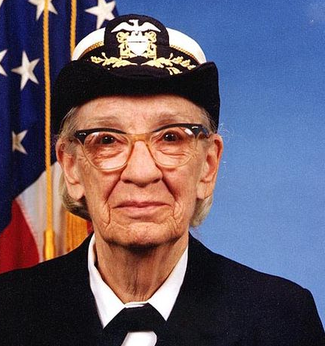
\includegraphics[width=0.86\linewidth]{hopper-original}\\[2pt]
  {\small\bfseries Original photograph}
\end{minipage}\hfill
\begin{minipage}[t]{0.30\textwidth}\centering
  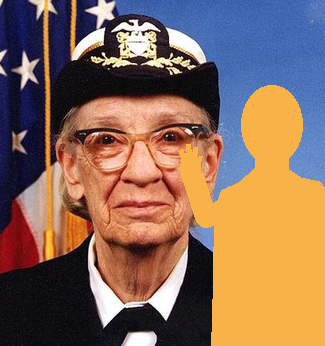
\includegraphics[width=0.86\linewidth]{hopper-front}\\[2pt]
  {\small\bfseries Stand-in drawn in front}
\end{minipage}\hfill
\begin{minipage}[t]{0.30\textwidth}\centering
  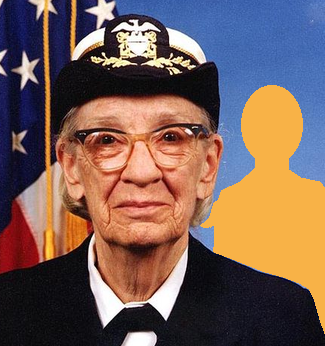
\includegraphics[width=0.86\linewidth]{hopper-behind}\\[2pt]
  {\small\bfseries Stand-in behind Hopper}
\end{minipage}
\caption{The same pose, drawn two ways. Follow the amber hand beside Hopper's glasses. It covers her face in the middle image and disappears behind her in the right image. The amber figure represents a visitor. All three panels are crops of the still-image test. Portrait by James S. Davis, U.S. Navy, 1984 [7].}
\end{figure}
\vfill

\begin{figure}[H]
\centering
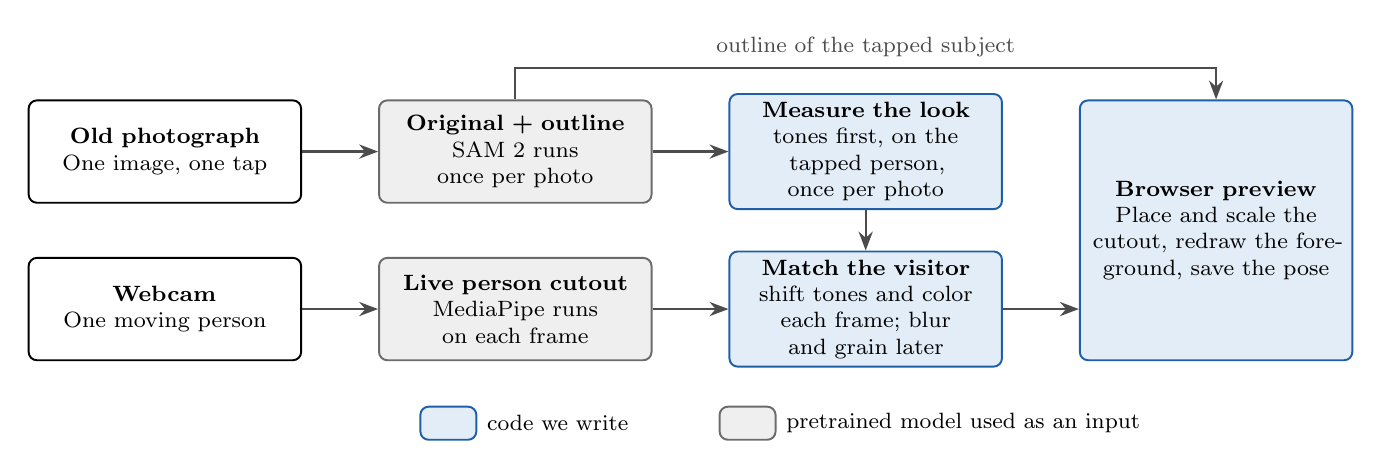
\begin{tikzpicture}[font=\footnotesize,
  box/.style={draw,rounded corners=3pt,minimum height=1.3cm,text width=3.25cm,align=center,inner sep=3pt,line width=0.7pt},
  o/.style={box,draw=ours,fill=oursfill},
  p/.style={box,draw=pre,fill=prefill},
  ar/.style={-{Stealth[length=2.4mm]},line width=0.8pt,black!70}]
  \node[box,fill=white] (photo) at (0,0) {\textbf{Old photograph}\\One image, one tap};
  \node[box,fill=white] (cam) at (0,-2) {\textbf{Webcam}\\One moving person};
  \node[p] (sam) at (4.45,0) {\textbf{Original + outline}\\SAM 2 runs\\once per photo};
  \node[p] (cutout) at (4.45,-2) {\textbf{Live person cutout}\\MediaPipe runs\\on each frame};
  \node[o] (measure) at (8.9,0) {\textbf{Measure the look}\\tones first, on the\\tapped person,\\once per photo};
  \node[o] (match) at (8.9,-2) {\textbf{Match the visitor}\\shift tones and color\\each frame; blur\\and grain later};
  \node[o,minimum height=3.3cm] (preview) at (13.35,-1) {\textbf{Browser preview}\\Place and scale the cutout, redraw the foreground, save the pose};
  \draw[ar] (photo) -- (sam);
  \draw[ar] (cam) -- (cutout);
  \draw[ar] (sam) -- (measure);
  \draw[ar] (cutout) -- (match);
  \draw[ar] (measure) -- (match);
  \draw[ar] (match.east) -- (match.east -| preview.west);
  \draw[ar] (sam.north) -- ++(0,0.4) -| (preview.north);
  \node[text=black!70,anchor=south] at ($(sam.north)!0.5!(preview.north)+(0,0.42)$) {outline of the tapped subject};
  \node[o,minimum height=0.42cm,text width=0.5cm] (k1) at (3.6,-3.45) {};
  \node[anchor=west] at (k1.east) {code we write};
  \node[p,minimum height=0.42cm,text width=0.5cm] (k2) at (7.4,-3.45) {};
  \node[anchor=west] at (k2.east) {pretrained model used as an input};
\end{tikzpicture}
\caption{How one frame is built. The old photograph fills the screen. The live cutout is first matched to the photo's look, then drawn at the chosen position and size. Inside the selected outline, the browser restores the old pixels so the original subject stays in front.}
\end{figure}
\vfill

\begin{figure}[H]
\centering
\begin{minipage}[t]{0.32\textwidth}\centering
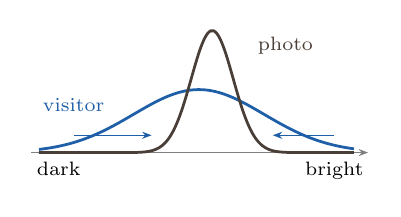
\begin{tikzpicture}[font=\scriptsize,x=1cm,y=1cm]
  \draw[black!50,line width=0.4pt,-{Stealth[length=1.2mm]}] (0,0) -- (4.28,0);
  \draw[ours,line width=1pt,domain=0.1:4.1,samples=60,smooth] plot (\x,{0.8*exp(-((\x-2.13)^2)/1.3778)});
  % The narrow peak is plotted only where it rises above the axis.
  \draw[ink,line width=1pt] (0.1,0) -- (1.3,0) -- plot[domain=1.3:3.3,samples=50,smooth] (\x,{1.55*exp(-((\x-2.3)^2)/0.1415)}) -- (3.3,0) -- (4.1,0);
  \draw[ours,line width=0.4pt,-{Stealth[length=1.2mm]}] (0.55,0.22) -- (1.53,0.22);
  \draw[ours,line width=0.4pt,-{Stealth[length=1.2mm]}] (3.85,0.22) -- (3.07,0.22);
  \node[ink] at (3.23,1.36) {photo};
  \node[ours] at (0.54,0.61) {visitor};
  \node[anchor=north] at (0.35,0) {dark};
  \node[anchor=north] at (3.85,0) {bright};
\end{tikzpicture}\\[3pt]
{\small\textbf{Tones and color.} Squeeze the visitor into the photo's range and tint.}
\end{minipage}\hfill
\begin{minipage}[t]{0.32\textwidth}\centering
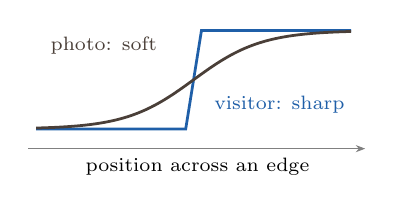
\begin{tikzpicture}[font=\scriptsize,x=1cm,y=1cm]
  \draw[black!50,line width=0.4pt,-{Stealth[length=1.2mm]}] (0,0) -- (4.28,0);
  \draw[ours,line width=1pt] (0.1,0.25) -- (2.0,0.25) -- (2.2,1.5) -- (4.1,1.5);
  \draw[ink,line width=1pt,domain=0.1:4.1,samples=60,smooth] plot (\x,{0.25+1.25/(1+exp(-(\x-2.1)/0.43))});
  \node[ours] at (3.19,0.56) {visitor: sharp};
  \node[ink] at (0.96,1.31) {photo: soft};
  \node[anchor=north] at (2.15,0) {position across an edge};
\end{tikzpicture}\\[3pt]
{\small\textbf{Softness.} Blur the visitor until its edges are as soft as the photo's.}
\end{minipage}\hfill
\begin{minipage}[t]{0.32\textwidth}\centering
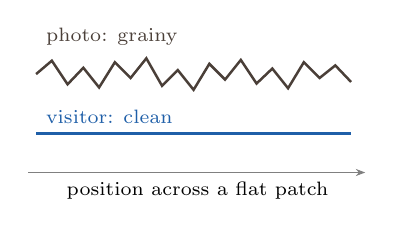
\begin{tikzpicture}[font=\scriptsize,x=1cm,y=1cm]
  \draw[black!50,line width=0.4pt,-{Stealth[length=1.2mm]}] (0,0) -- (4.28,0);
  \draw[ink,line width=0.9pt] (0.1,1.25) -- (0.3,1.42) -- (0.5,1.12) -- (0.7,1.33) -- (0.9,1.08)
    -- (1.1,1.40) -- (1.3,1.20) -- (1.5,1.45) -- (1.7,1.10) -- (1.9,1.30) -- (2.1,1.05)
    -- (2.3,1.38) -- (2.5,1.18) -- (2.7,1.43) -- (2.9,1.13) -- (3.1,1.32) -- (3.3,1.07)
    -- (3.5,1.40) -- (3.7,1.20) -- (3.9,1.36) -- (4.1,1.15);
  \draw[ours,line width=1pt] (0.1,0.5) -- (4.1,0.5);
  \node[ink,anchor=west,inner sep=0pt] at (0.22,1.73) {photo: grainy};
  \node[ours,anchor=west,inner sep=0pt] at (0.22,0.71) {visitor: clean};
  \node[anchor=north] at (2.15,0) {position across a flat patch};
\end{tikzpicture}\\[3pt]
{\small\textbf{Grain.} Add grain of the same strength to the visitor.}
\end{minipage}
\caption{What matching measures, drawn schematically. Dark lines are the old photo and blue lines are the live visitor before matching. Tones come first, measured on the tapped person and held fixed for the whole clip. Softness and grain follow only if viewers still notice them.}
\end{figure}
\vfill

\begin{figure}[H]
\centering
\begin{minipage}[t]{0.32\textwidth}\centering
  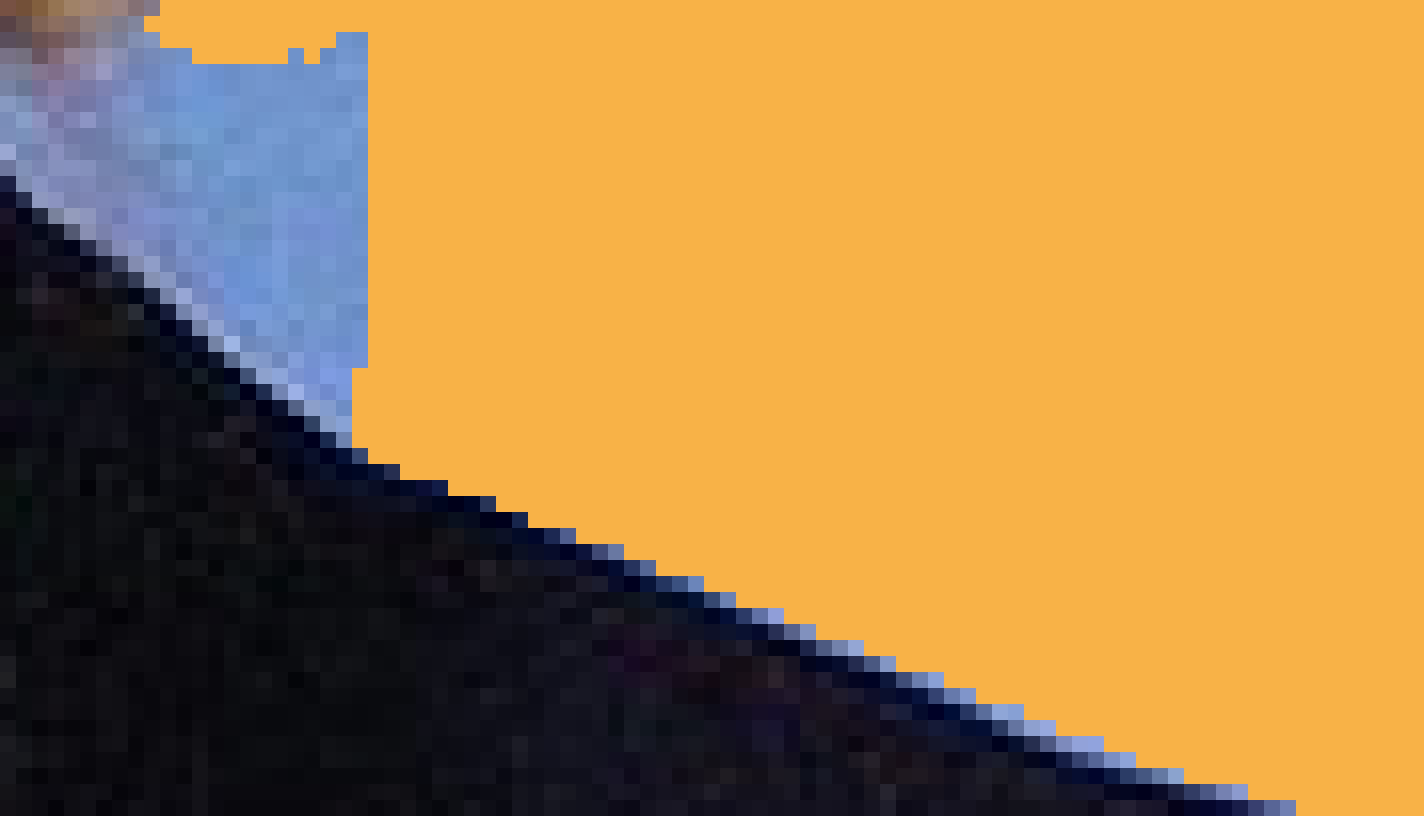
\includegraphics[width=\linewidth]{edge-traced}\\[2pt]
  {\small\bfseries Traced shoulder}
\end{minipage}\hfill
\begin{minipage}[t]{0.32\textwidth}\centering
  
\includegraphics[width=\linewidth]{edge-shifted}\\[2pt]
  {\small\bfseries Outline shifted 4 pixels}
\end{minipage}\hfill
\begin{minipage}[t]{0.32\textwidth}\centering
  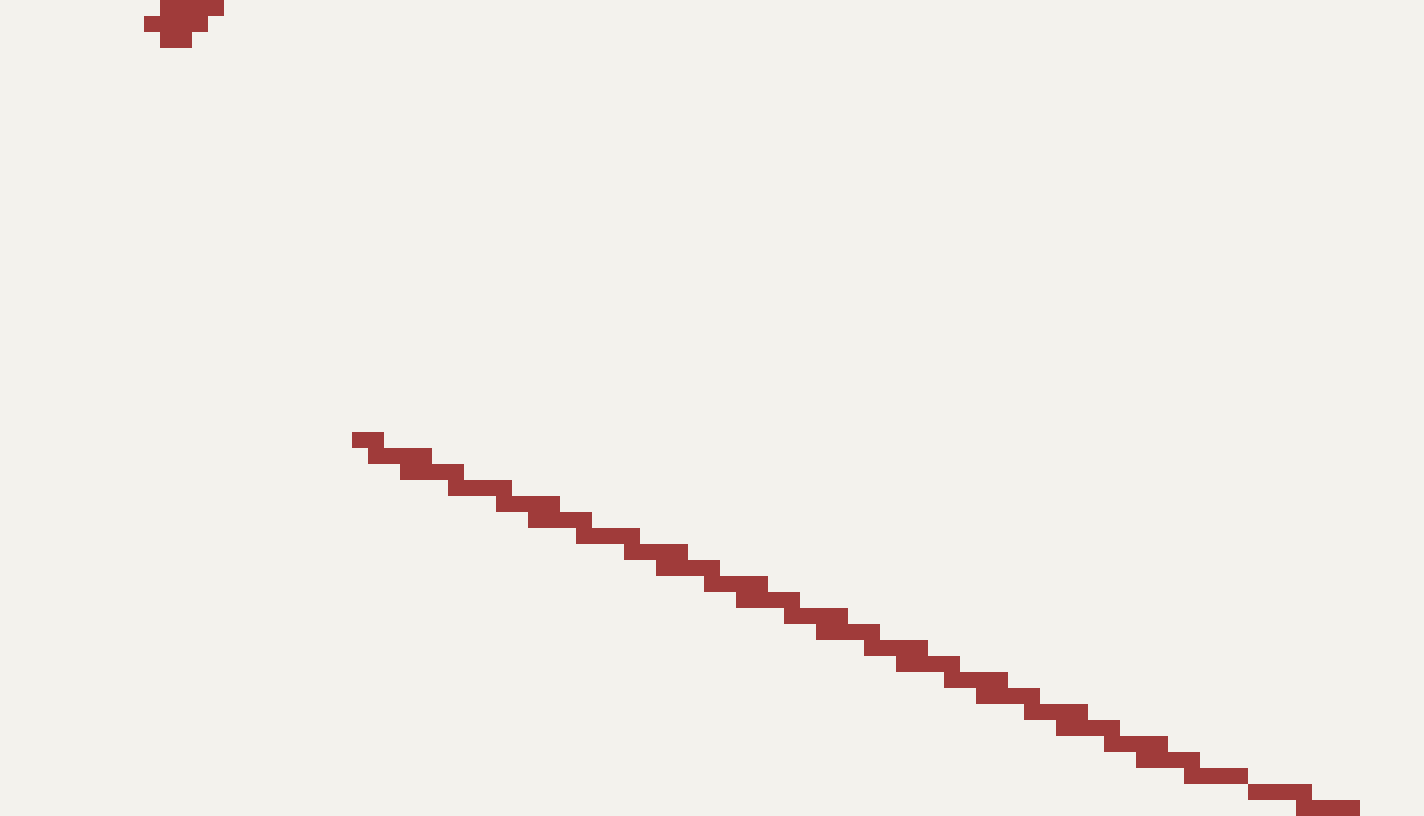
\includegraphics[width=\linewidth]{edge-changed}\\[2pt]
  {\small\bfseries Changed pixels in red}
\end{minipage}
\caption{An edge can look wrong even when most pixels match. The shifted outline pulls a strip of blue background over the amber figure. Across the full 384~$\times$~450 image, 414 of 172,800 pixels change. That is why we ask viewers to judge the moving edge and do not rely on pixel counts.}
\end{figure}

\clearpage
% =================== FIGURE PAGE 2 ===================
\vspace*{\stretch{1}}
\begin{figure}[H]
\centering
\begin{minipage}[t]{0.2345\textwidth}\centering
  \comparisonpanel{\person{83.1}{8}{1}{ink}{d}\person{71.2}{8}{1}{ours}{r}}\\[2pt]
  {\small\textbf{A: Flat overlay.} No foreground selection.}
\end{minipage}\hfill
\begin{minipage}[t]{0.2345\textwidth}\centering
  \comparisonpanel{\person{71.2}{8}{1}{ours}{r}\person{83.1}{8}{1}{ink}{d}}\\[2pt]
  {\small\textbf{B: Hand trace.} Trace one foreground subject.}
\end{minipage}\hfill
\begin{minipage}[t]{0.2345\textwidth}\centering
  \comparisonpanel{\person{71.2}{8}{1}{ours}{r}\person{83.1}{8}{1}{ink}{d}}\\[2pt]
  {\small\textbf{C: One tap.} Use SAM~2's top-ranked outline.}
\end{minipage}\hfill
\begin{minipage}[t]{0.2345\textwidth}\centering
  \comparisonpanel{\person{71.2}{8}{1}{matched}{r}\person{83.1}{8}{1}{ink}{d}}\\[2pt]
  {\small\textbf{D: One tap, matched.} The visitor takes on the photo's look.}
\end{minipage}
\caption{Planned comparison, shown schematically. A is shown only to explain what a flat overlay gets wrong. B shows how good the overlap can look given manual work. C is the time-saving hypothesis, judged blind against B. D is compared with C and with a simple fix such as grayscale. We will freeze the visitor's position, scale and recorded motion before comparing them.}
\end{figure}
\vspace{\stretch{2}}

\begin{figure}[H]
\centering
\small
\begin{tabularx}{\textwidth}{@{}>{\bfseries\raggedright\arraybackslash}p{0.177\textwidth}>{\raggedright\arraybackslash}X>{\raggedright\arraybackslash}p{0.2625\textwidth}@{}}
\toprule
Question & \textbf{Test} & \textbf{Target or output}\\
\midrule
What catches the eye first? & Show the same teammate joining two different photos, a black-and-white scan and a color group photo. Before saying what we changed, ask an open question: what caught your eye first? Repeat after each round of changes. & The first thing each viewer names, per photo. A problem named on both photos is fixed first.\\
\addlinespace
What does one tap cost in quality? & On each held-out photo, show the same lean as two unlabeled clips, B beside C, left/right randomized. Ask which looks more convincing and where they noticed a problem. Allow ``no difference.'' & Per photo: votes for each and ties, and where viewers saw an error the trace avoided. Show the failures.\\
\addlinespace
How much time does one tap save? & Three people new to the tool each set up one photo by tracing and another by tapping, without coaching. Record time to first outline, time to saved pose, and any correction or help. & The times side by side, split into outlining and positioning.\\
\addlinespace
Does matching beat a simple fix? & Show the same clip three ways: untreated (C), a simple fix, and our matching (D). The simple fix is grayscale on a black-and-white photo and one brightness and contrast shift on a color one. & Votes for each, and one photo where matching loses.\\
\addlinespace
Does it feel live? & On the demo laptop, count distinct camera frames segmented, matched and displayed in a 30-second run at 640~$\times$~480. Record device and browser. & At least 24 fresh frames per second.\\
\bottomrule
\end{tabularx}

\vspace{4pt}
\begin{tabularx}{\textwidth}{@{}>{\bfseries\raggedright\arraybackslash}p{0.177\textwidth}>{\raggedright\arraybackslash}X@{}}
\multicolumn{2}{@{}l}{\textbf{What we will bring to each check-in}}\\
\midrule
By 24 November & Updated proposal, two ten-second clips of the same teammate joining two different photos, each shown as original, untreated composite and best simple correction, what five viewers noticed, and a first one-tap attempt.\\
\addlinespace
By 4 December & Updated proposal, B and C compared on the 12 held-out photos, setup times from new users, the matching comparison, failure examples and the revised demo.\\
\bottomrule
\end{tabularx}
\caption{All thresholds are proposed targets. Viewers come from outside the team, at least six for each comparison, so we report counts and examples, not general claims. Comparison clips use identical placement and motion, with the B trace and the first C outline as made, before any repairs.}
\end{figure}
\vspace*{\stretch{1}}

\end{document}
